% ---- ETD Document Class and Useful Packages ---- %
\documentclass{ucetd}
%\usepackage{oneinchmargins}
\usepackage{times}
\usepackage{relsize}
\usepackage{enumerate}
\usepackage{graphicx}
\usepackage{url}
%\usepackage{color}
\usepackage[usenames,dvipsnames]{xcolor}
%\usepackage[pagebackref]{hyperref}
%\usepackage[bookmarks=false]{hyperref}

%\hypersetup{colorlinks=true,citecolor=OliveGreen,linkcolor=Maroon,urlcolor=NavyBlue}

%\hypersetup{colorlinks=true,
%citecolor=Maroon,
%linkcolor=Green,
%urlcolor=Maroon}

%\usepackage{breakurl}
\usepackage{setspace}
\usepackage{rotating}

\usepackage{floatflt}
\usepackage{wrapfig}
\usepackage{alltt}
\usepackage{epstopdf}
\usepackage{subfigure}

%\usepackage{listings}
%\usepackage{algorithm}
%\usepackage{algorithmic}

\usepackage{fancyvrb}
%\usepackage{ulem} % for strike out,  
% \em and \sout are now strikes, use \it for italic
% never do this because now all 
\renewcommand{\ttdefault}{cmtt}

%\usepackage{colortbl} % for table color
%\usepackage{pstricks} % for gray hline
%\input{colortab} % for gray hline (must include pstricks)
%\usepackage{array}



% make sure url bib break point does not
% give undefull hbox message and the break line 
% is really nice now
\usepackage{etoolbox}
\apptocmd{\thebibliography}{\raggedright}{}{}


% -----------------------------------------------------
\usepackage{rotating}

\usepackage{subfigure,epsfig,amsfonts}
\usepackage{natbib}
\usepackage{amsmath}
\usepackage{amssymb}
\usepackage{amsthm}


% ---------------------------------------------
% name abbrvs .. 
% ---------------------------------------------
\newcommand{\infokernel}{\mbox{infokernel}}
\newcommand{\unix}{{\sc Unix}}
\newcommand{\dare}{DARE}
\def \samc {\textsc{SamC}}
\def \sampro {\textsc{SamPro}}
\def \samzoo {\textsc{SamZoo}}
\def \sammr {\textsc{SamMr}}
\def \sammace {\textsc{SamMace}}
\def \samcass {\textsc{SamCass}}
\def \sameiger {\textsc{SamEiger}}
\def \modist {\textsc{Modist}}
\def \macemc {\textsc{MaceMC}}
\def \setsudo {\textsc{Setsudo}}
\def \prefail {\textsc{PreFail}}

\def \fate {\textsc{Fate}}
\def \late {\textsc{Late}}
\def \lights {\textsc{LigHTS}}

\def \taxdc {TaxDC}
\def \tdc {TaxDC}
\def \sck {\textsc{SCk}}
\def \cdb {\textsc{CbsDB}}
\def \cbs {CBS}

\newcommand{\ts}[1]{{\tt{\small#1}}}


\def \uuu {\textbf{\textcolor{Maroon}{\textbf{$\uparrow$}}}}
\def \uu {\textbf{\textcolor{Maroon}{\textbf{$\Uparrow$}}}}
% \def \nu {\textbf{\textcolor{Maroon}{\textbf{$\nearrow$}}}} % submission only

\def \sleep {\ts{sleep()}}

\newcommand{\num}[1]{\textcolor{red}{\textbf{#1}}}
\def \numOldDeepBugs {12} 
\def \numZkDeepBugs {7}   
\def \numMrDeepBugs {3}
\def \numCsDeepBugs {2}
\def \numZkNewBugs {1}
\def \numMrNewBugs {1}
\def \numNewBugs {2}
\def \numVersions {10}
\def \numLinesSamPro {10,886}
\def \numProtocols {7}
\def \numLinesRule {35}  
\def \numMaxBugSpeedUp {271x}  
\def \numAvgBugSpeedUp {33x}    
\def \numAvgExecTime {40}

\def \numMinRedRatio {37x}  
\def \numMaxRedRatio {166x}  
\def \numRedRatioExecs {3000}

%\newcommand{\mrb}[1]{MR-#1}
%\newcommand{\zkb}[1]{ZK-#1}
%\newcommand{\zk}[1]{ZooKeeper-#1}
%\newcommand{\mr}[1]{MapReduce-#1}
%\newcommand{\cs}[1]{Cassandra-#1}

\newcommand{\jira}[3]{\href{http://issues.apache.org/jira/browse/#1-#3}{#2-#3}}

\newcommand{\mrb}[1]{\jira{MAPREDUCE}{MR}{#1}}
\newcommand{\zkb}[1]{\jira{ZOOKEEPER}{ZK}{#1}}
\newcommand{\cab}[1]{\jira{CASSANDRA}{CA}{#1}}
\newcommand{\hbb}[1]{\jira{HBASE}{HB}{#1}}
\newcommand{\hdb}[1]{\jira{HDFS}{HD}{#1}}
\newcommand{\zk}[1]{\jira{ZOOKEEPER}{ZK}{#1}}
\newcommand{\mr}[1]{\jira{MAPREDUCE}{MR}{#1}}
\newcommand{\ca}[1]{\jira{CASSANDRA}{CA}{#1}}
\newcommand{\hb}[1]{\jira{HBASE}{HB}{#1}}
\newcommand{\hd}[1]{\jira{HDFS}{HD}{#1}}


\def \ll {\ts{L}}
\def \ff {\ts{F}}
\def \pri {\ts{pr}$_{i}$}
\def \prone {\ts{pr}$_{1}$}
\def \prtwo {\ts{pr}$_{2}$}
\def \prtri {\ts{pr}$_{3}$}

\def \ls {\ts{ls}}
\def \als {\ts{als}}
\def \rals {\ts{rals}}
\def \ralsi {\ts{rals}$_{i}$}
\def \ralsone {\ts{rals}$_{1}$}
\def \ralstwo {\ts{rals}$_{2}$}
\def \ralstri {\ts{rals}$_{3}$}
\def \rags {\ts{rags}}


\def \gs {\ts{gs}}
\def \ags {\ts{ags}}
\def \nn {\ts{N}}
\def \none {\ts{N1}}
\def \ntwo {\ts{N2}}
\def \ntri {\ts{N3}}
\def \nfour {\ts{N4}}
\def \mone {\ts{m}$_{1}$}
\def \mn {\ts{m}$_{n}$}
\def \mm {\ts{m}}
\def \fone {\ts{F1}}
\def \ftwo {\ts{F2}}
\def \ftri {\ts{F3}}
\def \ma {\ts{a}}
\def \mb {\ts{b}}
\def \mc {\ts{c}}
\def \md {\ts{d}}
\def \mx {\ts{m1}}
\def \my {\ts{m2}}
\def \xx {\ts{X}}
\def \pg {\ts{pg}}
\def \pl {\ts{pl}}
\def \pp {\ts{p}}
\def \pd {\ts{pd}}
\def \pi {\ts{pi}}
\def \pm {\ts{pm}}
\def \pc {\ts{pc}}

% ---------------------------------------------
% spaces
% ---------------------------------------------
\newcommand{\vtwenty}{\vspace{20pt}}
\newcommand{\vfifteen}{\vspace{15pt}}
\newcommand{\vten}{\vspace{10pt}}
\newcommand{\vfive}{\vspace{5pt}}
\newcommand{\vthree}{\vspace{3pt}}

\newcommand{\vmintwo}{\vspace{-2pt}}
\newcommand{\vminthree}{\vspace{-3pt}}
\newcommand{\vminfive}{\vspace{-5pt}}
\newcommand{\vminten}{\vspace{-10pt}}
\newcommand{\vminfifteen}{\vspace{-15pt}}
\newcommand{\vmintwenty}{\vspace{-20pt}}

% ---------------------------------------------
% overloaded commands
% ---------------------------------------------
\newcommand{\ub}[1]{\underline{{\bf #1}}}
\newcommand{\bquote}{\vspace{-0.25cm} \begin{quote}}
\newcommand{\equote}{\end{quote}\vspace{-0.2cm} }
\def \sec {\S}
\def \yes {$\surd$}

\def \nospace {
  \setlength{\itemsep}{0pt}
  \setlength{\parskip}{0pt}
  \setlength{\parsep}{0pt}
}


\newcommand{\supsection}[1]{\noindent{\Large{\bf #1}}\vten}

\newenvironment{enumerate2}{
  \begin{enumerate}
  \setlength{\itemsep}{1pt}
  \setlength{\parskip}{0pt}
  \setlength{\parsep}{0pt}
}{
  \end{enumerate}
}

\newenvironment{itemize2}{
  \begin{itemize}
 \renewcommand{\labelitemi}{-}
  \setlength{\itemsep}{1pt}
  \setlength{\parskip}{0pt}
  \setlength{\parsep}{0pt}
}{
  \end{itemize}
}

% \renewcommand\thesection{\Alph{section}}



% ---------------------------------------------
% note
% ---------------------------------------------
\newcommand{\hsg}[1]{\textcolor{red}{{\small {\bf (HSG: #1)}}}}
\newcommand{\tl}[1]{\textcolor{red}{{\small {\bf (TL: #1)}}}}
\newcommand{\pj}[1]{\textcolor{red}{{\small {\bf (PJ: #1)}}}}
\newcommand{\thanh}[1]{\textcolor{red}{{\small {\bf (THANH: #1)}}}}
\newcommand{\todo}[1]{\textcolor{red}{{\small {\bf (TODO: #1)}}}}
%\newcommand{\newtext}[1]{\textcolor{blue}{#1}}
\newcommand{\newtext}[1]{#1}
\newcommand{\bluetext}[1]{\textcolor{blue}{#1}}
\newcommand{\rbt}[1]{\textcolor{red}{\textbf{#1}}}
\newcommand{\notes}[1]{\textcolor{darkgray}{
{\footnotesize {\em (Notes: #1)}}}}






% ---------------------------------------------
% bullets
% ---------------------------------------------
\def \vvvnb {\vfifteen \noindent $\bullet$~}
\def \vvnb {\vten \noindent $\bullet$~}
\def \vnb {\vfive \noindent $\bullet$~}

\def \tb {\vspace{8pt}\nb}

\def \vvn {\vten \noindent}
\def \vn {\vfive \noindent}
\def \nb {\noindent $\bullet$~}
\def \ni {\noindent}



% ---------------------------------------------
% counters, steps, hypothesis, tasks
% ---------------------------------------------
\newcommand{\hypo}[1]{
\begin{quote}
\stepcounter{HYPO}{\bf Hypothesis \arabic{HYPO}:} 
{\em #1}
\end{quote}
}

\newcommand{\taskformat}[2]{#1\textsc{#2}}

\newcommand{\task}[3]{
\begin{quote}
\phantomsection
\hypertarget{task#1#2}{}
{\bf Task \taskformat{#1}{#2}:} 
{\em #3}
\end{quote}
}

\newcommand{\tasklink}[2]{\hyperlink{task#1#2}{\taskformat{#1}{#2}}}

\newcounter{HYPO}
\newcounter{TASK}

\newcommand{\rs}{{ResearchStaff$_1$}}
\newcommand{\raOne}{{\bf RA$_1$}}
\newcommand{\raTwo}{{\bf RA$_2$}}
\newcommand{\ndv}{{\bf NDV}}
\newcommand{\ug}{{\bf Undergrad$_1$}}


% ---------------------------------------------
% extra sections, pages
% ---------------------------------------------

\newcommand{\sssubsection}[1]{\vten\textbf{\large{\textsc{#1}}}}


\newcommand{\emptypage}{
\newpage
\thispagestyle{empty}
(empty page)
}


% ---------------------------------------------
% figs
% ---------------------------------------------
\newcommand{\myrotate}[1]{\begin{rotate}{90} {\bf #1} \end{rotate}}

\newcommand{\mycaption}[4][]{%
\ifthenelse{\equal{#1}{}}{
\begin{spacing}{0.95}
\caption{
\label{#2}
{\bf #3. } 
{\em #4}
}
\end{spacing}
}{
\begin{spacing}{0.95}
\caption[#1]{
\label{#2}
{\bf #3. } 
{\em #4}
}
\end{spacing}%
}}


% ---------------------------------------------
% general
% ---------------------------------------------
\newcommand{\eg}{\textit{e.g.}}
\newcommand{\ie}{\textit{i.e.}}
\newcommand{\etal}{\textit{et al.}}
\newcommand{\etc}{etc.}


\newcommand{\symstar}{$^{*}$}
\newcommand{\symtwostars}{$^{**}$}
\newcommand{\symthreestars}{$^{***}$}
\newcommand{\symdag}{$^{\dag}$}
\newcommand{\symddag}{$^{\ddag}$}


% ---------------------------------------------
% counters (\xxx\ cannot appear under figure caption)
% ---------------------------------------------
%\newcommand{\xxx}{{\bf XXX}} % --- no counter 
\newcounter{Xcounter}
\newcommand{\xxxreset}{\setcounter{Xcounter}{1}}
\newcommand{\xxx}{\textcolor{red}{\textbf{XXX$_{\arabic{Xcounter}}$}\stepcounter{Xcounter}}}

% settings
%\relscale{0.97}
%\setlength\parindent{0pt}
%\setlength\parskip{3pt}

\definecolor{fgray}{gray}{0.9}

%\newcommand{\hb}[1]{\jira{HBASE}{h}{#1}}
%\newcommand{\ca}[1]{\jira{CASSANDRA}{c}{#1}}

\newcounter{Fcounter}
\newcommand{\freset}{\setcounter{Fcounter}{1}}

\newcommand{\finding}[1]{
\begin{spacing}{1}
\findingTable{#1}
\end{spacing}
}

\newcommand{\findingTable}[1]{
%\vminfive
\begin{table}[h!]
\begin{center}
\begin{tabular}{|p{5in}|}
\hline
\rowcolor{fgray}
\findingBody{#1}\\
\hline
\end{tabular}
\end{center}
\end{table}
\vminfifteen
\vminfifteen
}

\newcommand{\findingBody}[1]{
\vfive
\begin{spacing}{1.5}
\textbf{Finding \#$\arabic{Fcounter}$:}
\stepcounter{Fcounter}
%\textit{#1}
#1 
\end{spacing}
\vminfifteen
}

\setcounter{Fcounter}{1}

\def \vvni {\vten \noindent}
\def \vni {\vfive \noindent}

\newcommand{\fev}[1]{\textcolor{Maroon}{\textit{#1}}}
\newcommand{\ev}[1]{\textcolor{gray}{\textbf{#1}}}

\newcommand{\bugbox}[1]{
\fbox{
\begin{minipage}{\textwidth}
\vspace{10pt}
\begin{quote}
#1
\end{quote}
\vspace{10pt}
\end{minipage}
}
}

\def \mytitle {SAMC: Semantic-Aware Model Checking for Fast Discovery of Deep Bugs in Cloud Systems}
%\usepackage[bookmarks=false]{hyperref}

%% Use these commands to set biographic information for the title page:
%\title{SAMC: Semantic-Aware Model Checking for Fast Discovery of Deep Bugs in Cloud Systems}
\title{\mytitle}
\author{Tanakorn Leesatapornwongsa}
\department{Computer Science}
\division{Physical Sciences}
\degree{Master's}
\date{2014}

%% Use these commands to set a dedication and epigraph text
%\dedication{Dedication Text}
%\epigraph{Epigraph Text}


\begin{document}
%% Basic setup commands
% If you don't want a title page comment out the next line and uncomment the line after it:
\maketitle
%\omittitle

% These lines can be commented out to disable the copyright/dedication/epigraph pages
\makecopyright
%\makededication
%\makeepigraph


%% Make the various tables of contents
\tableofcontents
\listoffigures
\listoftables

\acknowledgments
Acknowledgment here

\if 0
The first person I need to thank is my advisor and also one of the
thesis-committe members, Prof. Haryadi Gunawi. Without him, this thesis could
not happen. He guided me since the beginning to the end.  I have learned a lot
from him, not only research skills but also other soft skills to that surely will
benefit me during my future Ph.D. life. 

I also need to thank the other two committee members, Professor Shan Lu and
Professor Ravi Chugh that kindly to be my committee. Although I asked them in
very short manner, they still tried to schedule their valuable time to reivew
this thesis and give some feedback. I really appreciate their time.

And I need to thank my collegues, Mingzhe Hao, Pallavi Joshi (NEC Lab), and
Jeffrey Lukman (Surya University) for their hard working; and thank to my
friends, department faculty and staff to help me many things when I was working
on the thesis.

Lastly, there are five women I want to give big thanks to. The first most
important one is my mother, the woman who always supports me throughout my life.
The second one is Louise, my sweet fianc\'e; she always helps and supports me
during my hard time working on this thesis. And the other three are my lovely
sisters, Fon, Nuch, and Nid; they always make me feel good everytime I talk with
them.
\fi


\abstract
Cloud services must be accessible anytime and anywhere and not lose or corrupt
users' data (reliability), and scale as user base continues to grow
(scalability). Unfortunately, cloud-scale distributed systems behind the
services remain difficult to get right. Guaranteeing dependability has proven
to be challenging in these systems. In this proposal, We are tackling this
challenge. We try to unearth dependability bugs in cloud-scale distributed
systems, in the aspects of reliability and scalability

The first aspect that we focus is reliability. We find that one unsolved
reliability problem in cloud systems is distributed concurrency (DC) bugs. DC
bugs are caused by non-deterministic order of distributed events such as message
arrivals, faults, and reboots. Some interleavings of these events might not be
handled properly, and lead to catastrophic failures such as data loss, data
inconsistencies and downtimes. 

The last seven years have seen a rise of implementation-level distributed system
model checkers (dmck) for verifying the reliability of real distributed systems.
Existing dmcks however rarely exercise multiple faults due to the state-space
explosion problem, and thus do not address present reliability challenges of
cloud systems in dealing with complex faults. To scale dmck, we introduce
semantic-aware model checking (SAMC), a white-box principle that takes simple
semantic information of the target system and incorporates that knowledge into
state-space reduction policies.

For the second aspect, we focus on scalability. Scale surpasses the limit of a
single machine in meeting users' increasing demands of compute and storage.  On
the negative side, scale creates new development and deployment issues.
Developers must ensure that their algorithms and protocol designs to be
scalable. However, until real deployment takes place, unexpected bugs in the
actual implementations are unforeseen. We believe this new era of cloud-scale
distributed systems has given birth to a new type of bug: scalability bugs.
They are latent bugs that are scale-dependent; they only surface in large-scale
deployments only. Their presence jeopardizes systems reliability and
availability at scale.

We present \sck, a methodology that enables developers to scale-check
distributed systems and find scalability bugs on one machine. To colocate a
large number of nodes without sacrificing accuracy, we remove hardware
contentions with four novel strategies. And with these techniques, we achieve
high collocation factor.


\mainmatter
\chapter{Introduction}
\label{chp-intro}

As more data and computation move from local to cloud settings, cloud-scale
distributed systems such as scale-out storage systems \cite{Chang+06-BigTable,
DeCandia+07-Dynamo, Ghemawat+03-GoogleFS, Nightingale+12-FlatFDS}, computing
frameworks \cite{DeanGhemawat04-MapReduce, Murray+13-NaiadTimelyDataflow},
synchronization services \cite{Burrows06-Chubby, Hunt+10-ZooKeeperPaper}, and
cluster management services \cite{Hindman+11-Mesos, Kumar+13-Yarn} have become a
dominant backbone for many cloud services. Client-side software is getting
thinner and more heavily relies on the capability, reliability, and availability
of cloud systems. Users demand 24/7 dependability of cloud computing systems.
They must be accessible anytime and anywhere and not lose or corrupt users'
data, which means they must be reliable. Moreover, while user base continues
growing, they must be scalable also.

Unfulfilled dependability is costly. Some researchers estimate that 568 hours of
downtime at 13 well-known cloud services since 2007 to 2012 had an economic
impact of more than \$70 million~\cite{Essers12-70Million}. Others predict
worse: for every hour it is not up and running, a cloud service can take a hit
between \$1 to 5 million~\cite{Linthicum13-InfoworldCostOutages}.
Unfortunately, such cloud-scale distributed systems remain difficult to get
right. 
%
Cloud-scale distributed systems are getting more and more complex. New intricate
bugs continue to create dependability issues that cause major economic loss.
Guaranteeing dependability has proven to be challenging in these systems
\cite{Gunawi+11-FateDestini, Guo+11-Demeter, Wang+14-Exalt, Yang+09-Modist}.

In this proposal, we are tackling this challenge by answering these 2 questions,
(1) What bugs that harm the dependability, and (2) how do we test the systems to
unearth these bugs so developers can fix them? The first question is motivated
by that we do not have comprehensive knowledge about the bugs in distributed
systems. There are many bug studies on single-machine softwares
\cite{Jin+12-PerformanceBugs, Lu+08-ConcurrencyBugStudy, Palix+11-FaultsInLinux,
Sahoo+10-StudyBugsServerSoftware}, yet there are few formal bug studies on
distributed-systems softwares; they did not study in a great number and across
multiple types of systems \cite{Li+13-ScopeBugStudy, Xiao+14-NonDetMR}. We
believe that we need comprehensive understanding about cloud bugs to combat
them.

For the second question, we are motivated by the fact that in the past decade,
systems community has developed many testing techniques
\cite{Gunawi+11-FateDestini, Guo+11-Demeter, Wang+14-Exalt, Yang+09-Modist} to
find bugs in distributed systems, but these techniques still have limitations.
For example, \fate\ \cite{Gunawi+11-FateDestini} tests reliability of systems by
injecting faults, but it does not address concurrency in distributed systems.
\modist, which is a model checker, addresses concurrency, but it cannot work in
reasonable time when injecting multiple faults. Or Exalt, which is a framework
to test scalability, cannot be applied to CPU-intensive systems. 

We propose how to further the current testing techniques beyond the limitations
in this proposal. The proposal is arranged in this order: chapter \ref{chp-bg}
explains the problem being solved in detail and discusses related work, chapter
\ref{chp-plan} shows our research plans.
%
The proposal is a fusion of our previous work and our on-going work. It includes
cloud bug studies \cite{Gunawi+14-Cbs, Leesatapornwongsa+16-TaxDC},
semantic-aware model checking \cite{Leesatapornwongsa+14-Samc}, and scale check
methodology.


\section{Distributed Concurrency Bugs}

Distributed concurrency bugs (DC bugs) are bugs that caused by nondeterministic
orders of distributed events. Distributed events could be message arrivals,
hardware crashes/reboots, network timeout, \etc\ Cloud systems execute multiple
complicated distributed protocols concurrently (\eg, serving users' requests,
operating background tasks, and combined with untimely hardware failures), and
possible interleavings of the distributed events are beyond developers'
anticipation, which some interleavings might not be handled properly, and can
cause catastrophic failures such as data loss/inconsistency and downtimes.
Compared to the ``countless'' of efforts in combating ``local'' concurrency bugs
in multi-threaded software, DC bugs have not received the same amount of
attention within the research community.

Here is our contributions to combat DC bugs in systematic and comprehensive manners,

\begin{enumerate}

\item Semantic-Aware Model Checking (SAMC): we advance the state of the art of
model checking for distributed systems by adopting white-box approach to tackle
state-space explosion, the current limitation of model checking.

\item Taxonomy for DC bugs (\taxdc): we perform an in-depth study of more than
100 real-world DC bugs and built a first complet taxonomy for DC bugs. This
study will give insight to guide many future research work on DC bugs.

\end{enumerate}

The brief detail of these two works are discussed below.

\subsection{Semantic-Aware Model Checking}

One powerful method for discovering hidden DC bugs is the use of an
\textit{implementation-level distributed system model checker} (\textbf{dmck}).
A dmck can discover buggy interleavings that lead to DC bugs by reordering every
possibility of nondeterministic distributed events. The last ten years have seen
a rise of dmcks such as MaceMC, \modist, or Demeter. One big challenge faced by a
dmck is the state-space explosion problem (\ie, there are too many distributed
events to re-order). To address this, existing dmcks adopt a random walk or
basic reduction techniques such as dynamic partial order reduction (DPOR).
Despite these early successes, existing approaches cannot unearth many
real-world DC bugs, so we advance state of the art of dmck to combat DC bugs.

We start by addressing two limitations of existing dmcks. First, existing dmcks
treat every target system as a complete \textit{black box}, and perform
unnecessary reorderings of distributed events that would lead to the same states
(\ie, redundant executions). Second, they do not incorporate complex multiple
fault events (\eg, crashes, reboots, \etc) into their exploration strategies, as
such inclusion would exacerbate the state-space explosion problem.

To address these limitations, we introduce Semantic-Aware Model Checking
(\textbf{SAMC}), a novel white-box model checking approach that takes
\textit{semantic knowledge} of how distributed events (specifically, messages,
crashes, and reboots) are processed by the target system and incorporates that
to create reduction policies. The policies are based on sound reduction
techniques such as DPOR and symmetry. The policies tell SAMC not to re-order
some pairs of events such as message-message pairs, and message-crash pairs, yet
preserves soundness, because those cut out re-orderings are redundant, and
unnecessary to check.

SAMC can reproduce twelve old bugs in three cloud distributed systems
(Cassandra, Hadoop MapReduce, and ZooKeeper) involving 30-120 distributed events
and multiple crashes and reboots. Some of these bugs cannot be unearthed by
non-SAMC approaches, even after two days. SAMC can find the bugs up to 340 (49x
on average) faster compared to state-of-the-art techniques, it found two new
bugs in Hadoop MapReduce and ZooKeeper.

\subsection{DC Bug Study \& Taxonomy}

Bug and failure studies can significantly guide many aspects of dependability
research. Many researchers have recently employed formal studies on bugs and
failures \cite{Jin+12-PerformanceBugs, Li+13-ScopeBugStudy, Li+07-MemoryErrors,
Lu+08-ConcurrencyBugStudy, Sahoo+10-StudyBugsServerSoftware,
SridharanLiberty12-StudyDRAMFailures, Xiao+14-NonDetMR,
Yin+11-StudyConfErrors}.
%
However, we are not aware of any public large-scale DC-bug study, a recent study
from Microsoft analyzed the effect of distributed concurrency of workload and
only studied five DC bugs in MapReduce \cite{Xiao+14-NonDetMR}, and researchers
from NEC Labs dissected only network-failure-related DC bugs to study and did
not publicly release it \cite{Joshi+13-SetsudoTesting}.

In this dissertation, we fill the void by performing large-scale DC-bug study.
We study 104 real-world DC bugs from four various popular cloud-scale
distributed systems: Cassandra, HBase, Hadoop MapReduce/Yarn, and ZooKeeper. We
study DC bugs in all aspects including trigger, errors and failures, and fixes. 

For triggering conditions, we study DC bugs from two perspectives:
\begin{enumerate}

\item Timing conditions: For every DC bug, we identify the smallest set of
concurrent events E, so that a specific ordering of E can guarantee the bug
manifestation. This is similar to the interleaving condition for local
concurrency bugs.

\item Input preconditions: In order for those events in E to happen, regardless
of the ordering, certain inputs or fault conditions (\eg, node crashes) must
occur. This is similar to the input condition for local concurrency bugs.

\end{enumerate}
Understanding the triggering can help the design of testing tools that can
proactively trigger DC bugs, bug detection tools that can predict which bugs can
be triggered through program analysis, and failure prevention tools that can
sabotage the triggering conditions at run time.

Other than the trigger, we also look into errors and failures. From the
triggering conditions, we then scrutinize the first error that happens
immediately after. First errors are the pivotal point that bridges the
triggering and error-propagation process. We categorize first errors into {\em
local} errors and {\em global} errors, based on whether they can be observed
from the triggering node alone. 
%
And after the first errors, we track down to system failures that are noticeable
to users such as downtimes, lost/corrupted/inconsistent data, failed operations,
and degraded performance. Identifying errors and failures help failure diagnosis
get closer to disclosing bug triggering and root causes and help bug detection
get closer to accurately predict failures.

Lastly, we study how developers fix DC bugs to understand their fix strategies.
We want to see how different DC bug fixes compared to local concurrency bugs. In
general, we find that DC bugs can be fixed by either disabling the triggering
timing or changing the system's handling to that timing ({\em fix timing} vs.
{\em fix handling}). The former prevents concurrency with extra synchronization
and the latter allows concurrency by handling untimely events properly.
Understanding the fix strategies will help research on runtime failure
prevention and automatic bug fixing.

Our contribution from the study is the first complete taxonomy of DC bugs which
named \taxdc. \taxdc\ contains in-depth characteristics of DC bugs, stored in
the form of 2,083 classification labels and 4,528 lines of re-enumerated steps
to the bugs that we manually added. And as mentioned above, \taxdc\ can guide
various future research on combating DC bugs such as model checking, bug
detections, failure diagnosis, and failure prevention and fixing.


\section{Scalability Bugs}

Scalability bugs are a type of bug that newly born in the era of cloud
computing. These bugs are latent such that they do not surface in
small/medium-scale deployments, but only surface in large scale. They threaten
systems reliability and availability at scale. As we discussed above, cloud
backend needs to be scalable; algorithms and protocols in cloud distributed
systems are designed to be scalable. However, until real deployment takes place,
if developers do not have a large cluster to test their actual implementations,
unexpected bugs are unforeseen. 

\if 0
The following is our contribution to tackle this novel type of bugs:

\begin{enumerate}

\item Scalability bug study (SCB): we perform an in-depth study of 41
scalability bugs to analyze how an era of cloud computing gives a birth to a new
type of bugs that is scale dependent. This study is a bug benchmark for future
research on scalability aspect of cloud-scale distributed systems.

\item Scalability checking methodology for cloud-scale distributed systems
(\sck): we propose a methodology to help developers test and debug scalability
of systems in an economical way by colocate multiple nodes on one machine.

\end{enumerate}
\fi

To unearth latent scalability bugs, we need an effective and economic approach
to test the systems prior to deployments, but in order to do that, we need to
understand the nature of scalability bugs first. Unfortunately, we are not aware
of any study on scalability bugs at all, so in this dissertation, we perform a
study of scalability bugs to gain some foundational knowledge about them. We
study 41 bugs in seven systems including Cassandra, Couchbase, Hadoop MapReduce,
HBase, HDFS, Riak, and Voldemort. And here is our brief observations from the
study:

\begin{itemize}
\item Scalability bugs only appear at extreme scale (\eg, hundreds node).
\item Systems can be scalable in design, but not in practice.
\item Scalability bugs could be implementation specific and hard to predict.
\item Scalability bugs are caused from cascading impacts of ``not independent'' nodes.
\item It is long and difficult to debug large-scale.
\item Not all developers have large cluster to test the systems, especially in
open-source project.
\end{itemize}

These observations accentuate the need for scale-checking distributed system
{\em implementations} at {\em real scale}, not via simulation nor extrapolation.
The challenge of large-scale emulation is resource contention problem that is
nodes compete to consume resources (\eg, CPU, memory, and threds) and make test
outcome inaccurate.
%
In this context, we start a pilot work, \sck, a large-scale emulation that
allows developers to colocate hundreds nodes in one machines to test system
scalability, yet still get accurate testing results. \sck contains four
techniques to mitigate resource contention which we briefly describe below.

First, we introduce {\em processing illusion} (PIL), which replaces
scale-dependent CPU-intensive computations with \sleep without changing the
cluster behavior.  The insight behind PIL is that the key to computation is not
the intermediate results, but rather the execution time and eventual output.  To
make PIL feasible, we analyze the characteristics of functions that can take
PIL.  We employ pre-memoization and order determinism to record the output data
and execution time of PIL-replaceable functions.

In addition to PIL, we introduce other colocation strategies
that reduce unnecessary CPU and memory contentions, strategies such as
%
{\em single process cluster} (SPC), which runs the whole cluster
in a single process,
%
{\em global even driven architecture} (GEDA), which replaces
hundreds of threads in SPC with a few event-handler threads
shared by all nodes,
%
and {\em memory footprint reduction} (MFR), which removes high
system-specific memory footprints in our target systems.

We created \sck tools for Cassandra \cite{Lakshman+09-Cassandra}, Riak
\cite{RiakWeb}, and Voldemort \cite{VoldemortWeb}.
%
We scale-checked a total of \numProt\ protocols; \numProtCass\ Cassandra
(bootstrap, scale-out, decommission), \numProtRiak\ Riak (bootstrap+rebalance),
and \numProtVold\ Voldemort (rebalance) protocols.
%
To show the simplicity of developing \sck, we have migrated \sck to a total of
\numVers\ old and new releases (\numVersCass\ Cassandra, \numVersRiak\ Riak, and
\numVersVold\ Voldemort versions).
%
Across these versions, we have colocated 500 nodes and reproduced \numEval\ (old
and new) scalability bugs (5 Cassandra, 1 Riak, and 1 Voldemort bugs).

In summary, our contributions are:
%
\begin{enumerate} \item We present a method for scale-checking distributed
systems and reproducing the scalability bugs within.
%
\item We uncover the reasons why existing distributed systems are not easily
scale-checkable (\ie, the colocation bottlenecks).
%
\item We show the generality of \sck by applying the concept to three real-world
cloud-scale distributed systems.
%
\end{enumerate}

Overall, we believe that scalability bugs are new-generation bugs to combat in
modern cloud-scale distributed systems and \sck is one of the pilot solutions in
this new area of research.

\if 0
We see that most of the work \cite{Calotoiu+13-ApmScaleBug,
Laguna+15-DebugAtScale, Shudler+15-ExascaleLib, Wang+14-Exalt, Zhou+11-Vrisha,
Zhou+13-Wukong} focuses on the data path, mainly to validate the scalability of
read/write operations (linear throughput or stable latency as the cluster
scales). But scalability correctness however is not merely about the data path.
Distributed systems are full of ``control paths'' such as bootstrapping,
rebalancing, and adding/decommissioning nodes (scaling out/down). These
management protocols must modify cluster-wide metadata that lives in each node
in the system (\eg, ring partition table) to decide how data flows in the
cluster. Unfortunately, control path correctness is often overlooked, so in this
dissertation, we aim our attention to ``{\em control-plane scalability bugs}''.
\fi

\section{Summary of Contributions and Outline}

We summarize our contributions and present the outline for the rest of
dissertation below.

\begin{itemize}

\item Background

\item Semantic-aware model checking

\item Distributed concurrency bug study and taxonomy

\item Scalability bug study

\item Scalability checking methodology

\end{itemize}





\newcommand{\msg}[1]{{\tt{\textbf{#1}}}}



\chapter{Background}
\label{sec-mot}

\section{Overview}
This chapter gives a quick background on dmck and related terms,
followed with a detailed overview of the state of the art.  Then, we
present cases of deep bugs and motivate the need for dmck
advancements.





\section{DMCK Framework and Terms}
\label{mot-bgterms}




As mentioned before, we define {\em dmck} as  software model checker
that checks distributed systems directly at the implementation level.
Figure~\ref{fig-dmck} illustrates a dmck integration to a target
distributed system, a simple representation of existing dmck
frameworks~\cite{Guo+11-Demeter, Killian+07-LifeDeathMaceMC,
  Simsa+10-Dbug, Yang+09-Modist}.  The dmck inserts an interposition
layer in each node of the target system with the purpose of
controlling all important events (\eg, network messages, timeouts) and
preventing the target system to process the events until the dmck
enables them.  A main dmck mechanism is the permutation of events; the
goal is to push the target system into all possible ordering scenarios.
For example, the dmck can enforce \ts{abcd} ordering in one execution,
\ts{bcad} in another, and so on.



% List all the terms
We now provide an overview of basic dmck terms we use in this thesis
and Figure~\ref{fig-dmck}.
%
Each node of the target system has a {\em local state} (\ls),
containing many variables.  An {\em abstract local state} (\als) is a
subset of the local state; dmck decides which \als\ is important to
check.
%
The collection of all (and abstract) local states is the {\em global
  state} (\gs) and the {\em abstract global state} (\ags)
respectively.  
%
The {\em network state} describes all the {\em outstanding messages}
currently intercepted by dmck (\eg, \ts{abd}).
%
To model check a specific protocol, dmck starts a {\em workload
  driver} (which restarts the whole system, runs specific workloads,
\etc).  Then, dmck generates many (typically hundreds/thousands)
executions; an {\em execution} (or a {\em path}) is a specific
ordering of events that dmck enables (\eg, \ts{abcd}, \ts{dbca}) from
an initial state to a termination point.
%
A {\em sub-path} is a subset of a path/execution.
%
An {\em event} is an action by the target system that is intercepted
by dmck (\eg, a network message) or an action that dmck can inject
(\eg, a crash/reboot).
%
Dmck enables one event at a time (\eg, \ts{enable(c)}).
%
To permute events, dmck runs {\em exploration methods} such as
brute-force (\eg, depth first search) or random.  
%
%
As events are permuted, the target system enters hard-to-reach
states.  Dmck continuously runs state {\em checks} (\eg, safety 
checks) to verify the system's correctness.
%
To reduce the state-space explosion problem, dmck can employ {\em
  reduction policies} (\eg, DPOR or symmetry).  A policy is {\em
  systematic} if it does not use randomness or bug-specific knowledge.
%
In this work, we focus on advancing systematic reduction policies.




\input{mot-state}




\section{Deep Bugs}
\label{mot-deep}


\if 0
\tl{response to reviewer E, regarding fix time for each bug, and
encounter dep bugs that developers don't think are worth fixing.
    COMMENT: We can show the time since an issue was reported until it was
    closed, but we do not think that it tells us important information.
    Longer fix time does not mean it is harder to fix, it might mean
    developers asked for more information (e.g. Log files) and reporters
    need some time to gather that or wait until bugs happen again.  For the
    bugs that developers do not think they are worth to fix, yes we have
    seen some. The example of these bugs could be the wrong state of
    systems that eventually be detected and fixed by some error handle
    code. This kind of bugs makes a few nodes down for few minutes (before
    alive again) that developers think it is not that bad.}
\fi


% 94
% 54 total

% bug study
To understand the unique reliability challenges faced by cloud
systems, we performed a study of reliability bugs of three popular
cloud systems: ZooKeeper~\cite{Hunt+10-ZooKeeperPaper}, Hadoop
MapReduce~\cite{Kumar+13-Yarn}, and
Cassandra~\cite{Lakshman+09-Cassandra}.  We scanned through thousands
of issues from their bug repositories.  We then tagged complex
reliability bugs that can only be caught by a dmck (\ie, bugs that can
occur only on specific orderings of events).  We found 94
dmck-catchable bugs.\footnote[1]{Since this is a manual effort, we
  might miss some bugs.  We also do not report ``simple'' bugs (\eg,
  error-code handling) that can be caught by unit tests.}  Our major
finding is that 50\% of them are deep bugs (require complex
re-ordering of not only messages but also crashes and reboots).



% results, and observations
Figure~\ref{fig-deepbugs} lists the deep bugs found from our bug
study.  Many of them were induced by multiple crashes and reboots.
Worse, to reproduce the bugs, crash and reboot events must happen in a
specific order within a long sequence of events (\eg, the example bug
in \sec\ref{sec-intro}).  Deep bugs lead to harmful consequences (\eg,
failed jobs, node unavailability, data loss, inconsistency,
corruption), but they are hard to find.  We observe that since there
is no dmck that helps in this regard, deep bugs are typically found in
deployment (via logs) or manually, then they get fixed in few
weeks, but afterwards as code changes continuously, new deep bugs
tend to surface again.
% , as confirmed by cloud developers~\cite{ClouderaPC}.



\input{mot-summ}








\chapter{Semantic-Aware Model Checking}
\label{sec-samc}



% one paragraph about samc, 
\section{Overview}
Semantic-aware model checking (SAMC) is a white-box model checking
approach that takes semantic knowledge of how events (\eg, messages,
crashes, and reboots) are processed by the target system and
incorporates that information in reduction policies.  To show the
intuition behind SAMC, we first give an example of  a simple leader
election protocol. Then, we present SAMC architecture and our four
reduction policies.







% nothing here, see sam-overview









\section{An Example}
\label{sam-ex}

In a simple leader election protocol, every node broadcasts its vote to
reach a quorum and elect a leader.  Each node begins by voting for itself
(\eg, \ntwo\ broadcasts \ts{vote=2}).  Each node receives vote broadcasts
from other peers and processes every vote with this simplified code segment
below.  As depicted in the code segment below, if an incoming vote is less
than the node's current vote, it is simply discarded.  If it is larger, the
node changes its vote and broadcasts the new vote.

{\small
\begin{alltt}
  if (msg.vote < myVote) \{discard;\} 
  else \{myVote = msg.vote; broadcast(myVote);\}
\end{alltt}}



Let's assume \nfour\ with \ts{vote=4} is receiving three concurrent
messages with votes \ts{1}, \ts{2}, and \ts{3} from its peers.  Here,
a dmck with a black-box DPOR approach must perform 6 (3!) orderings
(\ts{123}, \ts{132}, and so on).  This is because a black-box DPOR
does {\em not} know the {\em message processing semantic} (\ie, how
messages will be processed by the receiving node).  Thus, a black-box
DPOR must treat all of them as dependent (\sec\ref{mot-state}); they
must be re-ordered for soundness.  However, by knowing the processing
logic above, a dmck can soundly conclude that all orderings will lead
to the same state; all messages will be discarded by \nfour\ and its local
state will not change.  Thus, a semantic-aware dmck can reduce the 6
redundant executions to just 1 execution.

The example above shows a scalability limitation of a black-box dmck.
Fortunately, simple semantic knowledge has a great potential in
removing redundant executions.  Furthermore, semantic knowledge can be
incorporated on top of sound model checking foundations such as DPOR
and symmetry, as we describe next.







\section{Architecture}
\label{sam-arch}





% figure, 3 mechanisms: abstractions (via history table), 
Figure~\ref{fig-samc} depicts the three levels of SAMC: sound
exploration mechanisms, reduction policies, and protocol-specific
rules.  SAMC is built on top of sound model checking foundations such
as DPOR~\cite{Flanagan+05-Dpor, Godefroid+96-Dpor} and
symmetry~\cite{Clarke+98-SymReduct, Prasad+00-SymBasedMc}.  We name
these foundations as mechanisms because a dmck must specify
accordingly what events are dependent/independent and symmetrical,
which in SAMC will be done by the reduction policies and
protocol-specific rules.






\begin{figure}[t]

\centerline{
%\includegraphics[height=1.4in]{F/empty.eps}
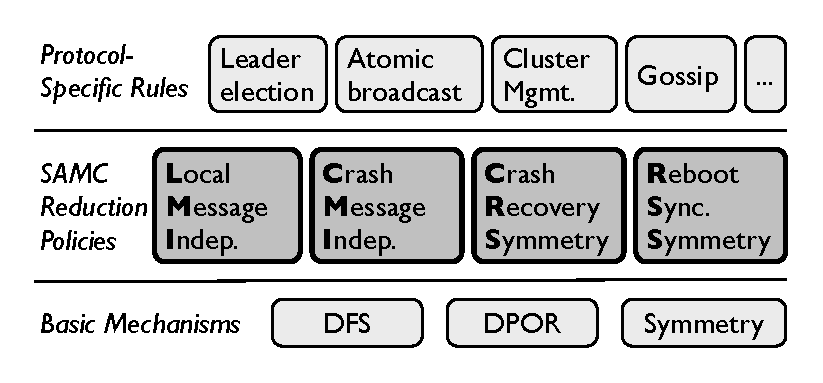
\includegraphics[height=2in]{F/samc/samc.eps}
}
\vminfive
\mycaption[SAMC Architecture]{fig-samc}{SAMC Architecture}{}
%\vminfive
\end{figure}

 % ------ fig samc

% 4 approaches and benefits
Our main contribution lies within our four novel {\em semantic-aware
  reduction policies}: local-message independence (LMI), crash-message
independence (CMI), crash recovery symmetry (CRS), and reboot
synchronization symmetry (RSS).  To the best of our knowledge, none of
these approaches have been introduced in the literature.  At the heart
of these policies are {\em generic event processing patterns} (\ie,
patterns of how messages, crashes, and reboots are processed by
distributed systems).  Our policies and patterns are simple and
powerful; they can be applied to many different distributed systems.  Testers
can extract the patterns from their target protocols (\eg,
leader election, atomic broadcast) and write protocol-specific
rules in few lines of code.

In the next section, we first present our four reduction policies
along with the processing patterns.  Later, we will discuss ways to
extract the patterns from target systems (\sec\ref{sam-extract}) and
then show the protocol-specific rules for our target systems
(\sec\ref{imp-targets}).





\section{Semantic-Aware Reduction Policies}
\label{sam-pol}



We now present four semantic-aware reduction policies that enable us to
define fine-grained event dependency/independency and symmetry beyond
what black-box approaches can do.




% policies
\input{sam-lmi}






\begin{figure}[t]

\centerline{
%\includegraphics[height=1.2in]{F/empty.eps}
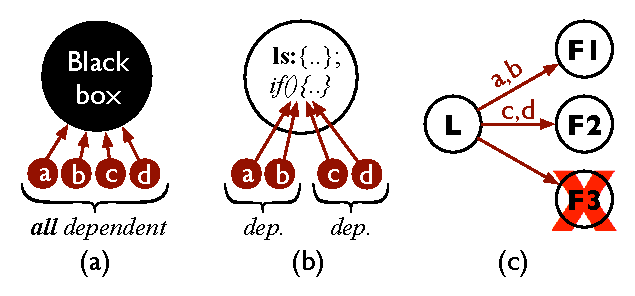
\includegraphics[height=2in]{F/pol/pol.eps}
}
\vminfive
\mycaption[LMI and CMI]{fig-pol}{LMI and CMI}{The figures
illustrate (a) a black-box approach, (b) local-message
independence with white-box knowledge, and (c)
crash-message independence.}
\vminten
\end{figure}



\input{sam-cmi}
\input{sam-crs}




\subsection{Reboot Synchronization Symmetry (RSS)}
\label{sam-rss}


Reboots are also essential to exercise (\sec\ref{mot-deep}), but if not
done carefully, will introduce more scalability problems.  Reboot reduction
policy is needed to help dmck inject reboots ``smartly''.  The intuition
behind reboot synchronization symmetry (RSS) is similar to that of CRS.
When a node reboots, it typically {\em synchronizes} itself with the peers.
However, a reboot will not lead to a new scenario if the current state of
the system is similar to the state when the node crashed.  To implement
RSS, we extract reboot-synchronization predicates and the corresponding
actions.  Since the overall approach is similar to CRS, we omit further
details.


In our experience RSS is extremely powerful.  For example, it allows
us to find deep bugs involving multiple reboots in the ZooKeeper
atomic broadcast (ZAB) protocol.  RSS works efficiently here because
reboots in ZAB are only interesting if the live nodes have seen new
commits (\ie, the dead node falls behind).  In contrast, a black-box
dmck without RSS initiates reboots even when the live nodes are in
similar states as in before the crash, prolonging the discovery of
deep bugs.





%\input{sam-ptop}
%\input{sam-pprio}




\input{sam-extract}

\section{Summary}
In this chapter, we have introduced semantic-aware model checking or SAMC (pronounced
``Sam-C''). We have explained a basic concept and architecture, and explained
semantic-aware reduction policies in detail, including how to construct them by
extracting semantic knowledge from the code.











\chapter{Implementation and Integration}
\label{sec-impl}

\section{Overview}
In this chapter, we first describe our SAMC prototype, \sampro, which we
built from scratch because existing dmcks are either
proprietary~\cite{Yang+09-Modist} or only work on restricted high-level
languages (\eg, Mace~\cite{Killian+07-LifeDeathMaceMC}).  We will then describe
\sampro\ integration to three widely popular cloud systems,
ZooKeeper~\cite{Hunt+10-ZooKeeperPaper}, Hadoop/Yarn~\cite{Kumar+13-Yarn},
and Cassandra~\cite{Lakshman+09-Cassandra}.  Prior to \sampro, there was no
available dmck for these systems; they are still tested via unit tests, and
the test code size is bigger than the main code, but the tests are far from
reaching deep bugs.






\section{\sampro}
\label{imp-pro}

\sampro\ is written in \numLinesSamPro\ lines of code in Java, which
includes all the components mentioned in Section~\ref{mot-bgterms} and
Figure~\ref{fig-dmck}.  The detailed anatomy of dmck has been
thoroughly explained in literature~\cite{Guerraoui+11-McNoNetwork,
  Guo+11-Demeter, Killian+07-LifeDeathMaceMC, Simsa+10-Dbug,
  Yang+09-Modist}, and therefore for brevity, we will not discuss many
engineering details.  We will focus on SAMC-related parts.

% access source code
We design \sampro\ to be highly portable; we do not modify the target code
base significantly as we leverage a mature interposition technology,
AspectJ, for interposing network messages and timeouts.
% local state
Our interposition layer also sends local state information to the
\sampro\ server.
% crashes and reboots
\sampro\ is also equipped with crash and reboot scripts specific to the
target systems.  The tester can specify a budget of the maximum number of
crashes and reboots to inject per execution.
% summ
\sampro\ employs basic reduction mechanisms and advanced reduction policies
as described before.
% checks
We deploy safety checks at the server (\eg, no two leaders).  If a
check is violated, the trace that led to the bug is reported and 
can be deterministically replayed in \sampro.
% other supports
Overall, we have built all the necessary features to show the case of
SAMC.  Other features such as intra-node thread
interleavings~\cite{Guo+11-Demeter}, scale-out
parallelism~\cite{Simsa+12-ScalablePOR}, and virtual clock for network
delay~\cite{Yang+09-Modist} can be integrated to \sampro\ as well.




\vten % orphan text

\section{Integration to Target Systems}
\label{imp-targets}


In our work, the target systems are ZooKeeper, Hadoop 2.0/Yarn, and
Cassandra.  ZooKeeper~\cite{Hunt+10-ZooKeeperPaper} is a distributed
synchronization service acting as a backbone of many distributed systems
such as HBase and High-Availability HDFS.  Hadoop
2.0/Yarn~\cite{Kumar+13-Yarn} is the current generation of Hadoop that
separates cluster management and processing components.
Cassandra~\cite{Lakshman+09-Cassandra} is a distributed key-value store
derived from Amazon Dynamo~\cite{DeCandia+07-Dynamo}.

In total, we have model checked \numProtocols\ protocols: ZooKeeper
leader election (ZLE) and atomic broadcast (ZAB), Hadoop cluster
management (CM) and speculative execution (SE), and Cassandra
read/write (RW), hinted handoff (HH) and gossiper (GS).  These
protocols are highly asynchronous and thus susceptible to message
re-orderings and failures.

Table~\ref{tab-policies} shows a real sample of protocol-specific
rules that we wrote.  Rules are in general very short; we only wrote
\numLinesRule\ lines/protocol on average.  This shows the simplicity
of SAMC's integration to a wide variety of distributed system protocols.




\begin{sidewaystable*}[t]
\begin{center}
{\small
%---------------------------------
\begin{tabular}{p{1.9in}|p{2in}|p{2.1in}|p{2in}} 


\multicolumn{1}{c|}{{\bf Local-Message}} &
\multicolumn{1}{c|}{{\bf Crash-Message}} &
\multicolumn{1}{c|}{{\bf Crash Recovery}} &
\multicolumn{1}{c}{{\bf Reboot Synchronization}}
\\

\multicolumn{1}{c|}{{\bf Independence (LMI)}} &
\multicolumn{1}{c|}{{\bf Independence (CMI)}} &
\multicolumn{1}{c|}{{\bf Symmetry (CRS)}} &
\multicolumn{1}{c}{{\bf Symmetry (RSS)}}
\\


\hline  % =====================================================

% ----------------------------------------------- ZLE, LMI (1)

\vminten
{\footnotesize
\begin{alltt}
bool pd : !newVote(m, s);

bool pm : newVote(m, s);

bool newVote(m, s) : {
 if (m.ep > s.ep) 
   return true; 
 else if (m.ep == s.ep)
  if (m.tx > s.tx) 
   return true;
  else if (m.tx == s.tx &&
           m.lid > s.lid) 
   return true;
}
\end{alltt}
}

& % ----------------------------------------------- ZLE, CMI (1)

\vminten
{\footnotesize
\begin{alltt}
bool pg (s, X) : 
 if (s.rl == F && X.rl == L)
  return true;
 if (s.rl == L && X.rl == F
     && !quorumAfterX(s)
  return true;
 if (s.rl == S && X.rl == S) 
  return true;

bool pl (s, X) :
 if (s.rl == L && X.rl == F 
     && quorumAfterX(s)) 
  return true;

bool quorumAfterX(s) :
  ret ((s.fol-1) >= 
        s.all/2);
\end{alltt}
}

& % ----------------------------------------------- ZLE, CRS (1)

\vminten
{\footnotesize
\begin{alltt}
bool pr1(s,C):
 if (s.rl == L && C.rl == F
     && quorumAfterX(s))
  return true;
rals1:\{rl,fol,all\};

bool pr2(s,C):
 if (s.rl == L && C.rl == F 
     && !quorumAfterX(s))
 return true;
rals2: \{rl,fol,lid,ep,tx,clk\}

bool pr3(s,C):
 if (s.rl == F && c.rl == L)
  return true;
rals3: \{rl,fol,lid,ep,tx,clk\}

bool pr4:
 if (s.rl == S)
  return true;
rals4: \{rl,lid,ep,tx,clk\}
\end{alltt}
}


& % ----------------------------------------------- ZLE, RSS (1)

\vminten
{\footnotesize
\begin{alltt}
bool ps1(s,R):
 if (s.rl == L)
  return true;
sals1: \{rl,lid,ep,tx,clk\}

bool ps2(s,R):
 if (s.rl == F)
  return true;
sals2: \{rl,lid,ep,tx,clk\}

bool ps3(s,R):
 if (s.rl == S && 
     s.clk > R.clk)
  return true;
sals3: \{rl,lid,ep,tx,clk\}

bool ps4(s,R):
 if (s.rl == S && 
     moreUpdated(s, R))
  return true;
sals4: \{rl,lid,ep,tx,clk\}

bool moreUpdated(s, R):
 if (R.ep > s.ep)
  return true;
 else if (R.ep == s.ep)
  if (R.tx > s.tx) 
   return true;
  else if (R.tx == s.tx)
   if (R.lid > s.lid)
    return true;
\end{alltt}
}

\end{tabular}
}
%---------------------------------
\end{center}
%
\vminfive
\mycaption[Protocol-Specific Reduction Rules for ZLE]{tab-policies}{Protocol-Specific Reduction Rules for ZLE}{
%
The code above shows the actual protocol-specific rules for
ZLE protocol.  These rules are the inputs to the four reduction policies.
%
Many variables are abbreviated (ep: epoch, tx: latest
transaction ID, lid: leader ID, rl: role, fol: follower count, all: total
node count, clk: logical clock, L: leading, F: following, S: searching,
X/C: crashing node, R: rebooting node). LMI \pc\ and \pi\ predicates are not 
used for ZLE, but used for other protocols. 
%
}
%\vminfive
\end{sidewaystable*}


\if 0
zle-specific rule = 49
zab-specific rule = 33
mapreduce: 35 ..
protocol average = 
\fi



\section{Summary}
In this chapter, we have talked about our prototype \sampro \; we have showed
technical detail how we built it and what cloud systems we targeted. In
addition, to give a sense of how protocol-specific reduction rules look like,
we have given an example of the rules for ZLE protocol.



\if 0
\input{imp-policy}
\input{imp-cases}

\fi







\chapter{Evaluation}
\label{sec-eval}


\section{Overview}
We now evaluate SAMC by presenting experimental results that answer the
following questions: 
\begin{enumerate}
\item How fast is SAMC in finding deep bugs compared to other state-of-the-art techniques?  
\item Can SAMC find new deep bugs?  
\item How much reduction ratio does SAMC provide?
\end{enumerate}

\if 0
(1) How fast is SAMC in finding deep bugs compared to
other state-of-the-art techniques?  (2) Can SAMC find new deep bugs?  (3)
How much reduction ratio does SAMC provide?
\fi

To answer the first question, we show SAMC's effectiveness in finding old
bugs.  For this, we have integrated \sampro\ to old versions of our target
systems that carry deep bugs: ZooKeeper v3.1.0, v3.3.2, v3.4.3, and v3.4.5,
Hadoop v2.0.3 and v2.2.0, and Cassandra v1.0.1 and v1.0.6.  To answer the
second question, we have integrated \sampro\ to two recent stable versions:
ZooKeeper v3.4.6 (released March 2014) and Hadoop v2.4.0 (released April
2014).  In total, we have integrated \sampro\ to \numVersions\ versions,
showing the high portability of our prototype.  Overall, our extensive
evaluation exercised more than 100,000 executions and used approximately 48
full machine days.




\if 0
\hsg{mention code coverage, and path coverage are hard
to quantify in Java code, or less priority}.
\fi




\input{eval-oldbugs}
\input{eval-newbugs}
\input{eval-reduce}
% \input{eval-future}

\section{Summary}
In this chapter we have evaluated SAMC by anwering these three questions:
\begin{enumerate}
\item How fast is SAMC in finding deep bugs compared to other state-of-the-art techniques?  
\item Can SAMC find new deep bugs?  
\item How much reduction ratio does SAMC provide?
\end{enumerate}
Table~\ref{tab-oldbugs} answers the first question by showing that SAMC is one
to two orders of magnitude faster. And to answer the second question, we can
also show that SAMC can find new bugs in cloud systems by integrating it to the
newest vesion code. For the third question, we have answered it by
table~\ref{tab-reduce} showing reduction ratio of 37x - 166x compare to bDP.





\if 0
\input{eval-coverage}
\input{eval-scale}
\input{eval-error}

\input{eval-complex}

\input{eval-deepness}

\input{eval-related}
\fi



\input{discuss}

\chapter{Related Work}
\label{sec-related}


\if 0
We now briefly discuss more related work on dmck and other approaches
to systems verification and testing.
\fi

\section{Existing Model Checkings}
% multiple failures
The threat of multiple failures to systems reliability already existed
since the P2P era; P2P systems are susceptible to ``churn'', the
continuous process of node joining and departing~\cite{Rhea+04-Churn}.
Many dmcks such as \macemc~\cite{Killian+07-LifeDeathMaceMC} and
CrystalBall~\cite{Yabandeh+09-CrystalBall} evaluate their approaches
on P2P systems.  Interestingly, we find that they mainly re-order join
messages.  To our understanding, based on their publications, they did
not inject and control node departures.  CrystalBall authors mentioned
about running churns, but only as part of their workloads, not as
events that the dmck can re-order.  This illustrates the non-triviality of
incorporating failures in dmck.

\section{Formal Model Checking Techniques}
% formal mc techniques .... 
Formal model checking foundations such as partial order
reduction~\cite{Flanagan+05-Dpor, Godefroid+96-Dpor},
symmetry~\cite{Clarke+98-SymReduct, Prasad+00-SymBasedMc}, and
abstraction~\cite{Clarke+94-McAbstract}, were established more than a
decade ago.  Here, classical model checkers require system models and
mainly focus on state-space reduction.  Implementation-level model
checkers on the other hand are expected to find real bugs in addition to
being efficient.

\section{Symbolic Execution}
% symbolic execution ...
Symbolic execution is another powerful formal method to verify
systems correctness.  Symbolic execution also faces an explosion
problem, specifically the path explosion problem.  A huge body of work
has successfully addressed the problem and made symbolic execution
scale to large (non-distributed) software
systems~\cite{Bucur+11-ParallelSymEx, Cadar+08-KLEE, Chipounov+11-S2e,
  Cui+13-RuleDirectedSymExec, Zamfir+10-Synthesis}.  Symbolic
execution and model checking can formally be combined into a more
powerful method~\cite{Burch+92-SymbolicMC}, however this concept has
not permeated the world of distributed systems; it is challenging to
track symbolic values across distributed nodes.


\section{Fault Injector}
% fault injector
Reliability bugs are often caused by incorrect handling of
failures~\cite{Gunawi+11-FateDestini, Gunawi+08-EIO}.  Fault-injection
testing however is challenging due to the large number of possible
failures to inject.  This challenge led to the development of
efficient fault-injection testing frameworks.  For example,
AFEX~\cite{Banabic+12-Blackbox} and
LFI~\cite{Marinescu+10-ExtensibleLFI} automatically prioritize
``high-impact targets'' (\eg, unchecked system calls).  These novel
frameworks target non-distributed systems and thus the techniques are
different than ours.


% distributed systems
Similarly, recent work highlights the importance of testing faults in
cloud systems (\eg, \fate~\cite{Gunawi+11-FateDestini},
\setsudo~\cite{Joshi+13-SetsudoTesting},
\prefail~\cite{Joshi+11-PreFail}, and OpenStack
fault-injector~\cite{Ju+13-FaultResOpenStack}).  As mentioned before
(\sec\ref{mot-state}), these frameworks are not a dmck; they cannot
re-order concurrent messages and failures and therefore cannot catch
distributed concurrency bugs systematically.



\section{Concurrency Bugs}
% local concurrency: Jula+08-DeadlockImmunity, Zhang+13-ConAir,
% Erickson+10-DataRaceKernel
The deep bugs we presented can be considered as concurrency bugs (in
distributed nature).  For non-distributed systems, there has been an
abundance of innovations in detecting, avoiding, and recovering from
concurrency bugs~\cite{Jin+12-CFix,
  Kasikci+13-CrowdRaceMob, 
  Lu+08-ConcurrencyBugStudy, 
  Veeraraghavan+11-ComplementarySchedules}.
They mainly target threads.  For dmck, we believe more advancements
are needed to unearth distributed concurrency bugs that still linger
in cloud systems.

\section{Geographically Distributed Systems}
% geo
\newtext{ Finally, the journey in increasing cloud dependability 
  is ongoing;  cloud systems face other issues such as bad error handling
  code~\cite{Yuan+14-Simplex}, performance failures~\cite{Do+13-Limplock},
  corruptions~\cite{Do+13-HARDFS}, and many others.  }
%
Exacerbating the
  problem, cloud systems are becoming larger and geographically
  distributed~\cite{Lloyd+11-Cops, Terry+13-PileusConsistencySLA,
    Zhang+13-TransactionChains}.  We believe cloud systems will observe
  more failures and message re-orderings, and therefore our work and future
  dmck advancements with the inclusion of failures will play an important
  role in increasing the reliability of future cloud systems.



\chapter{Conclusion and Future Work}
\section{Conclusion}
\label{sec-conclude}

Complex failures is a norm in cloud systems and deep bugs still linger in the
cloud.  To address present reliability challenges, dmcks must incorporate
complex failures, but due to the problem of state space explosion, existing
dmcks do not scale in this regard.  We strongly believe that without semantic
knowledge dmck hits a scalability wall.

In this thesis, we propose semantic-aware model checking (SAMC), a white-box
model checking approach that takes semantic knowledge and incorporates it in
reduction policies. 

We show a strong case that the SAMC principle can elegantly address this
scalability problem.  SAMC is simple and powerful; with simple semantic
knowledge, we show that dmcks can scale significantly.  We presented four
specific reduction policies, but beyond this, we believe our work triggers the
discussion of two important research questions: 
\begin{enumerate}
\item {\em What} other semantic knowledge can scale dmck?
\item {\em How} to extract white-box information from the target system? 
\end{enumerate}
We hope (and believe) that the SAMC principle can trigger future research in this
space.  



\section{Future}

\XXX{4 mins}

Well, that's all for my previous work. Now, I'll talk about my future work.

\subsection{Future Direction}

Here is my future direction

Toward DC bugs, TaxDC shows model checker needs to capture more events.

But to do that more challenges lie ahead, which I'll show.

For scalability bugs, they can happen in many axes, I just address one axe of
them. Many issues haven't been touched yet. I'll show you what are waiting for
us.

\subsection{DMCK}

Right now, SAMC doesn't address local computation timing, And also failure
model SAMC uses is only node fail-stop and reboot.

My first next step is advancing SAMC to capture local computation and expand
failure model.

The challenge here is this creates more events to re-order, and exacerbates
state space explostion.

So I will create more generic reduction policies to mitigate state space
explosion.

%In combating DC bugs, SAMC, a semantic aware model checker, leverage a domain
%specific knowledge to tackle state space explosion. 
%
%Right now, the generic patterns I exploit to build protocol-specific reduction
%policies are very simple. But this just scratches the surface of the power of
%semantic awareness. There are much more patterns and more reduction priciples
%waiting us to explore.
%
%So the next step on unearthing DC bugs is finding more patterns and creating
%more generic reduction policies, which will accelerate checking time.

%\subsection{AMC}

However, if you consider the current patterns I have here, they are very easy
to extract from the codebase.

Right now, we will have more reduction.

More reduction will find bugs faster, but that means extracting semantic
knowledge will be more complicated and harder.

This creates more burden on developers, and also introduce a chance of human
error.

And the error could leave bugs undetected..

My second step here will get rid of the burden of writing protocol-specific
policies by adopting program analysis to auto generate the policies.

%This will reduce the burden from developers and also the error.

\subsection{Scalability bugs}

Then let's look at scalability bugs. This class of bugs is new generation bugs
to combat in cloud-scale distributed systems.  And not much attention paid on
them. 

My vision here is to raise awareness on combating them.

On September this year, Cassandra developers started a new initiative to build
``Gossip 2.0'', by aiming at 1000 node cluster.

If they don't have a good way to test scalability, latent scalability bugs will
linger there. We might see a call for gossip 3.0 in a next few years.

%\subsection{4 axes}

As I said SCk is one of pilot works. It addresses only one axe of scalability,
which is scale of cluster.

From our cloud bug study, there are also

Scale of data

Scale of workload

And scale of failure

%SCk covers some part of scale of cluster. 

Previous work like Exalt covers some of scale of data. 

Many challenges lie ahead. In my future work, I'll adopt other techniques such
program analysis, to combat unsolved problems.



%\section{Conclusion}
\label{sec-conclude}

Complex failures is a norm in cloud systems and deep bugs still linger in the
cloud.  To address present reliability challenges, dmcks must incorporate
complex failures, but due to the problem of state space explosion, existing
dmcks do not scale in this regard.  We strongly believe that without semantic
knowledge dmck hits a scalability wall.

In this thesis, we propose semantic-aware model checking (SAMC), a white-box
model checking approach that takes semantic knowledge and incorporates it in
reduction policies. 

We show a strong case that the SAMC principle can elegantly address this
scalability problem.  SAMC is simple and powerful; with simple semantic
knowledge, we show that dmcks can scale significantly.  We presented four
specific reduction policies, but beyond this, we believe our work triggers the
discussion of two important research questions: 
\begin{enumerate}
\item {\em What} other semantic knowledge can scale dmck?
\item {\em How} to extract white-box information from the target system? 
\end{enumerate}
We hope (and believe) that the SAMC principle can trigger future research in this
space.  


%
\section{Future}

\XXX{4 mins}

Well, that's all for my previous work. Now, I'll talk about my future work.

\subsection{Future Direction}

Here is my future direction

Toward DC bugs, TaxDC shows model checker needs to capture more events.

But to do that more challenges lie ahead, which I'll show.

For scalability bugs, they can happen in many axes, I just address one axe of
them. Many issues haven't been touched yet. I'll show you what are waiting for
us.

\subsection{DMCK}

Right now, SAMC doesn't address local computation timing, And also failure
model SAMC uses is only node fail-stop and reboot.

My first next step is advancing SAMC to capture local computation and expand
failure model.

The challenge here is this creates more events to re-order, and exacerbates
state space explostion.

So I will create more generic reduction policies to mitigate state space
explosion.

%In combating DC bugs, SAMC, a semantic aware model checker, leverage a domain
%specific knowledge to tackle state space explosion. 
%
%Right now, the generic patterns I exploit to build protocol-specific reduction
%policies are very simple. But this just scratches the surface of the power of
%semantic awareness. There are much more patterns and more reduction priciples
%waiting us to explore.
%
%So the next step on unearthing DC bugs is finding more patterns and creating
%more generic reduction policies, which will accelerate checking time.

%\subsection{AMC}

However, if you consider the current patterns I have here, they are very easy
to extract from the codebase.

Right now, we will have more reduction.

More reduction will find bugs faster, but that means extracting semantic
knowledge will be more complicated and harder.

This creates more burden on developers, and also introduce a chance of human
error.

And the error could leave bugs undetected..

My second step here will get rid of the burden of writing protocol-specific
policies by adopting program analysis to auto generate the policies.

%This will reduce the burden from developers and also the error.

\subsection{Scalability bugs}

Then let's look at scalability bugs. This class of bugs is new generation bugs
to combat in cloud-scale distributed systems.  And not much attention paid on
them. 

My vision here is to raise awareness on combating them.

On September this year, Cassandra developers started a new initiative to build
``Gossip 2.0'', by aiming at 1000 node cluster.

If they don't have a good way to test scalability, latent scalability bugs will
linger there. We might see a call for gossip 3.0 in a next few years.

%\subsection{4 axes}

As I said SCk is one of pilot works. It addresses only one axe of scalability,
which is scale of cluster.

From our cloud bug study, there are also

Scale of data

Scale of workload

And scale of failure

%SCk covers some part of scale of cluster. 

Previous work like Exalt covers some of scale of data. 

Many challenges lie ahead. In my future work, I'll adopt other techniques such
program analysis, to combat unsolved problems.



% Format a LaTeX bibliography
\makebibliography

% Figures and tables, if you decide to leave them to the end
%\input{figure}
%\input{table}

\end{document}


